% Chapter 3

\chapter{Induced interaction} % Main chapter title

\label{Chapter3} % For referencing the chapter elsewhere, use \ref{Chapter3} 

\lhead{Part II. \emph{Kitaev wires}}
\chead{Chapter 3. \emph{Induced interaction}} % This is for the header on each page - perhaps a shortened title

%----------------------------------------------------------------------------------------
We wish to calculate an effective Hamiltonian for the fermions. In this chapter we therefore derive the induced interaction between the fermions on the wires. First stop is to look at the effective interaction between the fermions on the wires and the bosons in the condensate.

\section{Effective Bose-Fermi interaction}
The effective interaction between the fermions ($F$) and the bosons ($B$) is modelled by a delta function potential with strength $g_{BF}$: $V(\mathbf{r})=g_{BF}\delta(\mathbf{r})$. This is physically realistic, because the atom-atom interaction range is short range compared to the interparticle distance. This means, that the interaction Hamiltonian for the effective pair interaction reads:
\begin{equation}
H_{BF}^\text{int}  = \int d^3 r d^3 r' \; \psi_F^\dagger(\mathbf{r}) \psi_B^\dagger(\mathbf{r}')V(\mathbf{r}-\mathbf{r}')\psi_B(\mathbf{r}')\psi_F(\mathbf{r}) = g_{BF}\int d^3 r \; \psi_F^\dagger(\mathbf{r}) \psi_B^\dagger(\mathbf{r})\psi_B(\mathbf{r})\psi_F(\mathbf{r}),
\label{eq.HintBF}
\end{equation}
where $\psi_i(\mathbf{r})$ is the field operator for the $i$-particles, and so $\psi_i^\dagger(\mathbf{r})$ creates a particle at position $\mathbf{r}$.\footnote{The subscript $BF$ specifies, that it is the Hamiltonian for the interaction between bosons and fermions.} Notice, that there is no factor of $1/2$ in front of the integrals. As noted in section \ref{sec.secondquantization} the factor of $1/2$ should be omitted, when the particles are distinguishable, as fermions and bosons most certainly are. 

\begin{figure} 
\begin{center}  
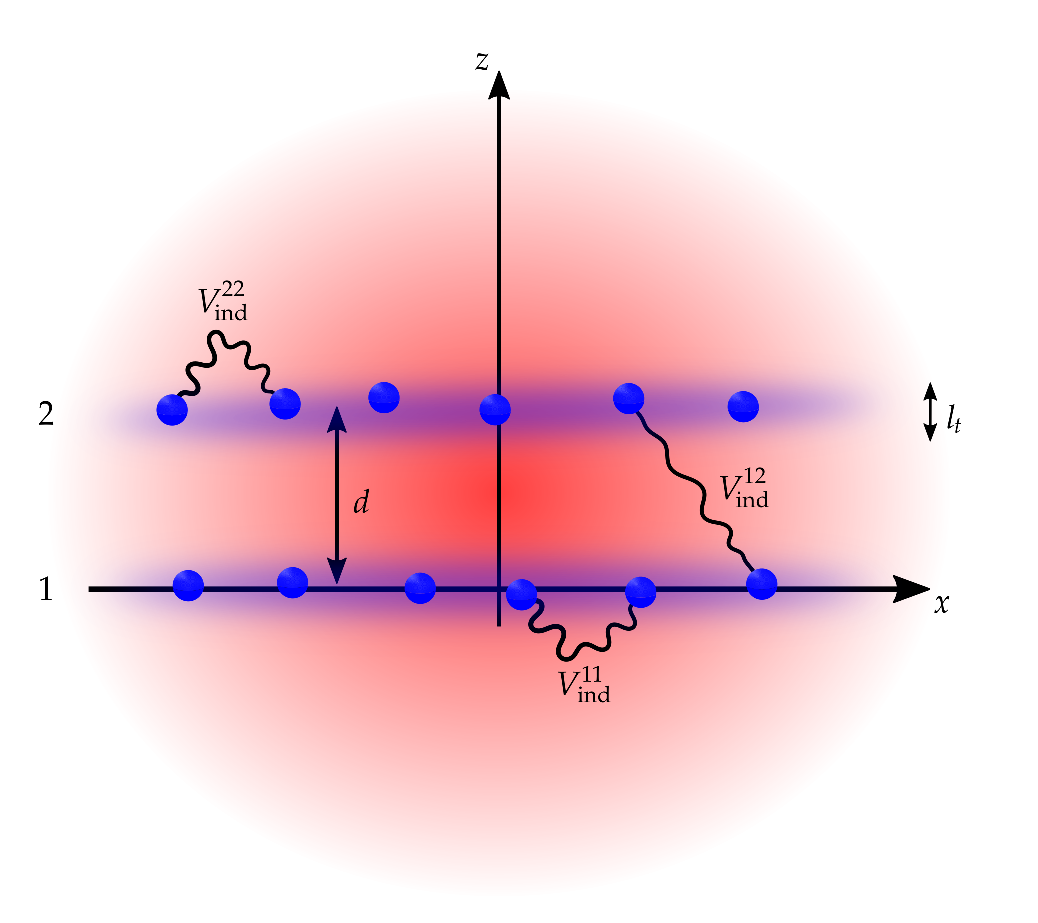
\includegraphics[width=0.7\columnwidth]{gasandwiresfancy2.eps}  
\caption{Sketch of the double wire system. The fermion gas is shown in blue. The BEC is shown in red. Fermion wire 1 is placed along the $x$-axis, wire 2 parallel hereto at $z = d$. The wires are confined by a harmonic potential with trapping frequency $\omega_t$. The resulting width of the wires is $l_t = 1/\sqrt{m_F\omega_t}$. By making $(k_Fl_t)^2 \ll 1$ we trap the fermions in the harmonic ground state, $\phi_0$, with respect to the perpendicular directions to the wires. The distance between the wires is $d$. We assume, that $l_t / d \ll 1$, so that the wires are truly distinguishable. The fermions and bosons interact through a contact potential. This results in induced interactions, $V^{ij}_{\text{ind}}$, between the fermions represented by the wiggly lines.}  
\label{fig.gasandwires}  
\end{center}    
\end{figure}

The physical setup of the system is depicted in figure \ref{fig.gasandwires}. The fermions ($F$) are confined to two one-dimensional wires. The first one is placed along the $x$-axis, the second at $z = d, y = 0$. The confinement is provided by two harmonic traps, $V_t(\mathbf{r}_{\perp}) = \frac{1}{2}m_F\omega_t^2r_{\perp}^2$, with $\mathbf{r}_{\perp} = (y, z)$. Hence, the two traps have the same trapping frequency, $\omega_t$. In this connection we have two central assumptions. Firstly, we require that the fermions are trapped in the ground state with respect to the perpendicular directions. The energy gap from the ground state to the first excited state is $\omega_t$. Hence, by making $\omega_t$ sufficiently large we trap the fermions in the lowest lying state, $\phi_0$, along the two wires. Specifically, the typical energy of the fermions is the free gas Fermi energy $\epsilon_{F,0} = \frac{k_F^2}{2m_F}$. Hence, we require $\frac{\epsilon_{F,0}}{\omega_t} \ll 1$. Using the trapping width $l_t = \frac{1}{\sqrt{m_F\omega_t}}$, we can also express this as $(k_Fl_t)^2 \ll 1$. One might be afraid of violating the Pauli exclusion principle in this context. However, the states in the $x$-direction are allowed to be different, and so we can symmetrize in the $y$- and $z$-directions.

The second assumption is, that the distance between the wires is much larger than the trapping width of the wires, $l_t$. Hence, $l_t/d \ll 1$. This is done, so that we can actually talk about distinguishable wires of fermions. This leads to the following expansion in momentum eigenstates:
\begin{equation}
\psi_F(x,\mathbf{r}_\perp) = \frac{1}{\sqrt{\mathcal{L}}}\sum_p \text{e}^{ipx} \left[\phi_0(\mathbf{r}_\perp) c_{1,p} + \phi_0(\mathbf{r}_\perp - \mathbf{d}) c_{2,p}\right], \hspace{0.5cm} \psi_B(\mathbf{r}) = \frac{1}{\sqrt{\mathcal{V}}}\sum_{\mathbf{k}} \text{e}^{i\mathbf{k}\cdot \mathbf{r}} b_\mathbf{k}, 
\end{equation}  
with $\phi_0(\mathbf{r}_\perp) = \frac{1}{\sqrt{\pi}l_t}\exp\left(-\frac{r_\perp^2}{2l_t^2}\right)$ the harmonic ground state with respect to the perpendicular directions and $\mathbf{d} = d\cdot\hat{z}$ the position of wire 2. $c^\dagger_{j,p}$ creates a fermion in wire $j$ with momentum $p$. $b^\dagger_\mathbf{k}$ creates a boson with momentum $\mathbf{k}$.  We assume, that the wires are truly distinguishable. This means that all anticommutators like $\{c_{1,p}, c^\dagger_{2,p'}\}$ vanish. Inserting these expressions into $H_{BF}^\text{int}$ yields in total four terms. However, the cross terms where a fermion is annihilated in one wire and created in the other are proportional to the integral: $\int d^2 r_\perp \phi_0(\mathbf{r}_\perp)\phi_0(\mathbf{r}_\perp-\mathbf{d}) \simeq 0$. The integral is negligible, because by assumption $l_t/d \ll 1$. The terms arising from interactions with fermions in wire 1 are:
\begin{equation}
H_{BF, 1}^{\text{int}} = \frac{g_{BF}}{\mathcal{LV}}\int d^3 r \sum_{p,p',q,q'}\sum_{\mathbf{k}_{\perp},\mathbf{k}_{\perp}'}\text{e}^{i((p-p')+(q-q'))x} \phi^2_0(\mathbf{r}_{\perp})\text{e}^{i(\mathbf{k}_{\perp} - \mathbf{k}_{\perp}')\cdot \mathbf{r}_\perp} c^\dagger_{1,p'} b^\dagger_{q',\mathbf{k}_\perp'}b_{q,\mathbf{k}_\perp}c_{1,p}. \nonumber
\end{equation}
The integral over $x$ yields the factor $\mathcal{L}\delta_{p-p',q'-q}$, implying total momentum conservation along the wire. The integral over $\mathbf{r}_\perp$ gives the Fourier transform of $\phi_0^2(\mathbf{r}_\perp)$. Since $\phi_0$ is a gaussian, the Fourier transform is as well. Explicitly: $\int d^2 r_\perp \; \phi^2_0(\mathbf{r}_{\perp})\text{e}^{i(\mathbf{k}_{\perp}-\mathbf{k}_{\perp}')\cdot \mathbf{r}_\perp} = \text{e}^{-\frac{l_t^2}{4}(\mathbf{k}_{\perp}-\mathbf{k}_{\perp}')^2}$. Taking the sum over $q'$ forces $q' = p - p' + q$. In total:
\begin{align}
H_{BF, 1}^{\text{int}} &= \frac{g_{BF}}{\mathcal{V}}\sum_{p, p', q} \sum_{\mathbf{k}_\perp, \mathbf{k}_\perp'} \text{e}^{-\frac{l_t^2}{4}(\mathbf{k}_\perp-\mathbf{k}_\perp')^2} c^\dagger_{1, p'} b^\dagger_{p - p' + q, \mathbf{k}_\perp'} b_{q, \mathbf{k}_\perp}c_{1, p} \nonumber \\
                  &= \frac{g_{BF}}{\mathcal{V}}\sum_{p_1, p_2, q} \sum_{\mathbf{k}_\perp, \mathbf{k}_\perp'} \text{e}^{-\frac{l_t^2}{4}(\mathbf{k}_\perp-\mathbf{k}_\perp')^2} c_{1, p_2 - q}^\dagger b_{p_1 + q, \mathbf{k}_\perp'}^\dagger b_{p_1, \mathbf{k}_\perp}c_{1, p_2}.
\end{align}
The last line is obtained by appropriate renaming. To be very specific: $p_1, p_2$ and $q$ are in the $x$ direction, along wire 1, whilst $\mathbf{k}_\perp'$ and $\mathbf{k}_\perp$ are momenta in the $(y,z)$-plane, hence perpendicular to wire 1. The interactions with fermions in wire 2 yields a very similar result. The only alteration is, that $\phi_0(\mathbf{r}_\perp) \to \phi_0(\mathbf{r}_\perp - \mathbf{d})$. The above Fourier transformation therefore yields an additional phase of $\text{e}^{i(\mathbf{k}_\perp - \mathbf{k}_\perp')\cdot \mathbf{d}}$. In total the interaction Hamiltonian hereby becomes:
\begin{align}
H_{BF}^\text{int} = \frac{g_{BF}}{\mathcal{V}}\sum_{p_1,p_2,q} \sum_{\mathbf{k}_\perp, \mathbf{k}_\perp'} & \text{e}^{-\frac{l_t^2}{4}(\mathbf{k}_\perp - \mathbf{k}_\perp')^2}\left[ c^\dagger_{1,p_2-q} b^\dagger_{p_1+q, \mathbf{k}_\perp'} b_{p_1,\mathbf{k}_\perp}c_{1,p_2} \right. \hspace{0.5cm} \feynmandiagram [small, inline, horizontal=a to b] {
  a -- [fermion] i2 [particle=\( 1 \)],
  i1 [particle=\( 1 \)] -- [fermion] a, 
  a -- [photon] b,
  f1 [particle=\( b \)] -- [fermion] b -- [fermion] f2 [particle=\( b \)],
}; \nonumber \\
& \left. + \text{e}^{i(\mathbf{k}_\perp - \mathbf{k}_\perp')\cdot \mathbf{d}}c_{2,p_2-q}^\dagger b_{p_1+q, \mathbf{k}_\perp'}^\dagger b_{p_1,\mathbf{k}_\perp}c_{2,p_2} \right]. \hspace{0.5cm} 
\feynmandiagram [small, inline, horizontal=a to b] {
  a -- [fermion] i2 [particle=\( 2 \)],
  i1 [particle=\( 2 \)] -- [fermion] a, 
  a -- [photon] b,
  f1 [particle=\( b \)] -- [fermion] b -- [fermion] f2 [particle=\( b \)],
};
\end{align}
This interaction Hamiltonian defines the fundamental vertices between fermions and bosons shown to the right. It shows, that a scattering event in wire 1 is associated with the factor $g_{BF} \text{e}^{-\frac{l_t^2}{4}(\mathbf{k}_\perp - \mathbf{k}_\perp')^2}$, and that the corresponding scattering in wire 2 has an extra factor of $\text{e}^{i(\mathbf{k}_\perp - \mathbf{k}_\perp')\cdot \mathbf{d}}$. Note that the transverse momentum, $\mathbf{k}_{\perp}$, is not conserved in these scattering events. This is due to the mixed dimensionality of the system. An obvious thing to do now would be to take the very narrow wire width limit, $l_t \to 0$. However, as we shall see later, it will be crucial to keep the trapping frequency finite, at least at the present stage.  

\section{Induced interaction between the fermions} \label{sec.1D3Dinducedinteraction}
We are interested in the properties of the fermion wires. We therefore calculate the induced interaction between the fermions mediated by the bosons in the condensate. This is later inserted into an effective Hamiltonian for the fermions. 

\subsection{Feynman diagrams} \label{subsec.Feynmandiagrams}
The bosons are assumed to be in a weakly interacting Bose-Einstein condensate (BEC), so that Bogoliubov theory applies. We are further only interested in the weak coupling limit.\footnote{There is a small fraction in nonzero momenta states, which is neglected. It would be necessary to include this for stronger interactions.} In turn we assume, that the bosons are essentially unaffected by the presence of the fermions. This is physically reasonable, because the fermions only occupies space along one-dimensional wires in the three-dimensional BEC. Hence, the density of the bosons $n_B$ is uniform and independent of the presence of the fermions. 

In a more general setup, one would have to calculate contributions from increasing orders in the underlying bare interaction between the bosons and fermions leading to a socalled $T$-matrix. This will not be pursued here. We will write the coupling strength as $g_{BF} = \frac{2\pi a_{BF}}{m_r}$, with $m_r = \frac{m_Fm_B}{m_B + m_F}$ the reduced mass, and $a_{BF}$ the effective scattering length. In a formally precise manner one can expand the $T$-matrix in orders of $a_{BF}$. From this analysis, it is clear that the smallness of the coupling strength is equivalent to demanding both $(n_Ba_{BF}^3)^{1/3}\ll 1$ and $n_Fa_{BF} \ll 1$. We can also argue for this by a dimensional analysis. $a_{BF}$ has dimension of length, and so we need the relevant parameters of dimension per length to get a unitless expression. There are two relevant length scales in the problem. One is the boson-boson distance, $n_B^{-1/3}$. The other is the fermion-fermion distance, $n_F^{-1}$. An increase in either of these distances leads to more fermion-boson interactions. Therefore, we should assume both $(n_Ba_{BF}^3)^{1/3} \ll 1$ and $n_Fa_{BF}\ll 1$. In this weak coupling limit we can safely take interactions only up to second order in $g_{BF}$. This means, that the four leading order diagrams for the fermion-fermion interaction mediated by the bosons are the ones showed in figure \ref{fig.feynmandiagrams}. 

\begin{figure}
\center
\begin{tikzpicture}[scale=0.25]
  \begin{feynman}[small]
    \vertex (number1) {\( (1) \)};
    \vertex [above left=of number1] (fermion1) {\(1, \tilde{p}_1 \)};
    \vertex [above right=of fermion1] (a);
    \vertex [below right=of a] (fermion2) {\(1, \tilde{p}_1 + \tilde{q}\)}; 
    \vertex [above=of a] (b);
    \vertex [above left=.5cm of b] (boson1);
    \vertex [left=.2cm of b] (boson1note)   {\( \sqrt{n_B} \)}; 
    \vertex [above= of b] (c);
    \vertex [below left=.5cm of c] (boson2);
    \vertex [left=.2cm of c] (boson2note) {\( \sqrt{n_B} \)};
    \vertex [above= of c] (d);
    \vertex [above left=of d] (f3) {\(1, \tilde{p}_2\)};
    \vertex [above right=of d] (f4) {\(1, \tilde{p}_2 - \tilde{q}\)};
 
    \diagram* {
      (number1) -- [opacity=0.0] (fermion1) -- [fermion] (a) -- [fermion] (fermion2),
      (a) -- [photon, edge label'=\(g_{BF}\)] (b),
      (b) -- [dashed] (boson1),
      (b) -- [blue, fermion, out=30, in=-30, edge label' = {\(-\tilde{q}, \mathbf{k}_\perp \)}] (c),
      (c) -- [dashed] (boson2),
      (c) -- [photon, edge label'=\(g_{BF}\)] (d),
      (d) -- [anti fermion] (f3),
      (d) -- [fermion] (f4)
    };
  \end{feynman}
\end{tikzpicture}
\begin{tikzpicture}
  \begin{feynman}[small]
    \vertex (number2) {\( (2) \)};
    \vertex [above left=of number2] (fermion1) {\(1, \tilde{p}_1 \)};
    \vertex [above right=of fermion1] (a);
    \vertex [below right=of a] (fermion2) {\(1, \tilde{p}_1 + \tilde{q}\)}; 
    \vertex [above=of a] (b);
    \vertex [above left=.5cm of b] (boson1);
    \vertex [left=.2cm of b] (boson1note)   {\( \sqrt{n_B} \)}; 
    \vertex [above= of b] (c);
    \vertex [below left=.5cm of c] (boson2);
    \vertex [left=.2cm of c] (boson2note) {\( \sqrt{n_B} \)};
    \vertex [above= of c] (d);
    \vertex [above left=of d] (f3) {\(1, \tilde{p}_2\)};
    \vertex [above right=of d] (f4) {\(1, \tilde{p}_2 - \tilde{q}\)};
 
    \diagram* {
      (number2) -- [opacity=0.0] (fermion1) -- [fermion] (a) -- [fermion] (fermion2),
      (a) -- [photon, edge label'=\(g_{BF}\)] (b),
      (b) -- [dashed] (boson1),
      (b) -- [blue, anti fermion, out=30, in=-30, edge label' = {\(\tilde{q}, \mathbf{k}_\perp \)}] (c),
      (c) -- [dashed] (boson2),
      (c) -- [photon, edge label'=\(g_{BF}\)] (d),
      (d) -- [anti fermion] (f3),
      (d) -- [fermion] (f4)
    };
  \end{feynman}
\end{tikzpicture}
\begin{tikzpicture}
  \begin{feynman}[small]
    \vertex (number3) {\( (3) \)};
    \vertex [above left=of number3] (fermion1) {\(1, \tilde{p}_1 \)};
    \vertex [above right=of fermion1] (a);
    \vertex [below right=of a] (fermion2) {\(1, \tilde{p}_1+\tilde{q}\)}; 
    \vertex [above=of a] (b);
    \vertex [above left=.5cm of b] (boson1);
    \vertex [left=.2cm of b] (boson1note)   {\( \sqrt{n_B} \)};  
    \vertex [above= of b] (c);
    \vertex [below left=.5cm of c] (boson2);
    \vertex [left=.2cm of c] (boson2note) {\( \sqrt{n_B} \)};
    \vertex [above= of c] (d);
    \vertex [above left=of d] (f3) {\(1, \tilde{p}_2\)};
    \vertex [above right=of d] (f4) {\(1, \tilde{p}_2-\tilde{q}\)};
 
    \diagram* {
      (number3) -- [opacity=0.0] (fermion1) -- [fermion] (a) -- [fermion] (fermion2),
      (a) -- [photon, edge label'=\(g_{BF}\)] (b),
      (b) -- [dashed] (boson1),
      (b) -- [blue, majorana, out=30, in=-30, edge label' = {\(\tilde{q}, \mathbf{k}_\perp \)}] (c),
      (c) -- [dashed] (boson2),
      (c) -- [photon, edge label'=\(g_{BF}\)] (d),
      (d) -- [anti fermion] (f3),
      (d) -- [fermion] (f4)
    };
  \end{feynman}
\end{tikzpicture}
\begin{tikzpicture}
  \begin{feynman}[small]
    \vertex (number4) {\( (4) \)};
    \vertex [above left=of number4] (fermion1) {\(1, \tilde{p}_1 \)};
    \vertex [above right=of fermion1] (a);
    \vertex [below right=of a] (fermion2) {\(1, \tilde{p}_1+\tilde{q}\)}; 
    \vertex [above=of a] (b);
     \vertex [above left=.5cm of b] (boson1);
    \vertex [left=.2cm of b] (boson1note)   {\( \sqrt{n_B} \)}; 
    \vertex [above= of b] (c);
    \vertex [below left=.5cm of c] (boson2);
    \vertex [left=.2cm of c] (boson2note) {\( \sqrt{n_B} \)};
    \vertex [above= of c] (d);
    \vertex [above left=of d] (f3) {\(1, \tilde{p}_2\)};
    \vertex [above right=of d] (f4) {\(1, \tilde{p}_2-\tilde{q}\)};
 
    \diagram* {
      (number3) -- [opacity=0.0] (fermion1) -- [fermion] (a) -- [fermion] (fermion2),
      (a) -- [photon, edge label'=\(g_{BF}\)] (b),
      (b) -- [dashed] (boson1),
      (b) -- [blue, anti majorana, out=30, in=-30, edge label' = {\(\tilde{q}, \mathbf{k}_\perp \)}] (c),
      (c) -- [dashed] (boson2),
      (c) -- [photon, edge label'=\(g_{BF}\)] (d),
      (d) -- [anti fermion] (f3),
      (d) -- [fermion] (f4)
    };
  \end{feynman}
\end{tikzpicture}
\caption{Feynman diagrams for the induced interaction in wire 1. Since the interaction is weak, we can neglect all other Feynman diagrams than (1)-(4). Diagrams (1) and (2) stems from the normal Green's function $G_{11}$. Diagrams (3) and (4) stems from the anormalous Green's functions $G_{12}$ and $G_{21}$. The diagrams have the same form for the interwire interaction. The only difference is, that $g_{BF}$ carries an extra phase factor for interactions in wire 2. } 
\label{fig.feynmandiagrams}
\end{figure}

Notice that the bosons of the BEC, shown with dashed lines, carry a factor of $\sqrt{n_B}$. This simply describes a boson coming out of or into the condensate. Further $\tilde{p}_j = (p_j, i\omega_{m_j})$, with $\omega_{m} = (2m + 1)\pi kT$ a fermionic Matsubara frequency, and $\tilde{q} = (q, i\omega_q )$, with $\omega_q = \omega_{m_1} - \omega_{m_2}$ a bosonic Matsubara frequency. The blue lines in the diagrams are the normal and anormalous Bogoliubov phonon Green's functions derived in subsection \ref{sec.BECGreens}. The diagrams can intuitively be understood as follows. A fermion in one wire interact with a boson in the condensate. This creates a ripple in the condensate described by one of the Green's functions. This ripple reaches a second fermion in one of the two wires, where the momentum of the ripple is transferred to. Further, a boson is "returned" to the condensate. In a more technical way we say, that the fermions interact by exchanging a condensate Bogoliubov phonon.   

From here on out the analysis depends on the mixed dimensionality of the problem. Let us first focus on the induced interaction between two fermions in wire 1. The perpendicular momentum $\mathbf{k}_{\perp}$ is not conserved in the Bose-Fermi scattering. Therefore, we have to integrate over this. Since the momentum of the incoming and outgoing boson in each diagram is 0 we simply get a factor of $g_{BF}\; \text{e}^{-\frac{l_t^2}{4}k_\perp^2}$ \textit{twice}. Collecting all factors gives us the four contributions from the four diagrams (1)-(4) to the fermion-fermion induced interaction $V_{\text{ind}}^{11}$: 
\begin{align}
V^{11}_{\text{ind}, 1}(q,i\omega_q) &= n_Bg_{BF}^2\int\frac{d^2k_\perp}{(2\pi)^2}G_{11}(-q,\mathbf{k}_\perp,-\omega_q)\text{e}^{-\frac{l_t^2}{2}k_\perp^2}, \nonumber \\
V^{11}_{\text{ind}, 2}(q,i\omega_q) &= n_Bg_{BF}^2\int\frac{d^2k_\perp}{(2\pi)^2}G_{11}(q,\mathbf{k}_\perp,\omega_q)\text{e}^{-\frac{l_t^2}{2}k_\perp^2}, \nonumber \\
V^{11}_{\text{ind}, 3}(q,i\omega_q) &= n_Bg_{BF}^2\int\frac{d^2k_\perp}{(2\pi)^2}G_{12}(q,\mathbf{k}_\perp,\omega_q)\text{e}^{-\frac{l_t^2}{2}k_\perp^2}, \nonumber \\
V^{11}_{\text{ind}, 4}(q,i\omega_q) &= n_Bg_{BF}^2\int\frac{d^2k_\perp}{(2\pi)^2}G_{12}(q,\mathbf{k}_\perp,\omega_q)\text{e}^{-\frac{l_t^2}{2}k_\perp^2}. 
\end{align}
We notice, that the last two give the same contribution in this weak interacting limit.\footnote{This would \textit{not} be the case, when including higher order terms.} The 11 superscript means, that it is for two fermions in wire 1. Summing up the four contributions gives us the frequency dependent induced interaction $V^{11}_{\text{ind}}$ for fermions in wire 1:
\begin{equation}
V^{11}_{\text{ind}}(q,i\omega_q) = g_{BF}^2\int\frac{d^2k_\perp}{(2\pi)^2}\; \chi_\text{BEC}(q,\mathbf{k}_\perp,i\omega_q)\text{e}^{-\frac{l_t^2}{2}k_\perp^2}, 
\label{eq.V11indXBEC}
\end{equation}
with $\chi_\text{BEC}(\mathbf{k},i\omega_q) = \frac{k^2}{m_B}\frac{n_B}{(i\omega_q)^2 - E_{B,k}^2}$ the socalled density-density correlation function of the BEC. It now becomes clear, why we had to retain a nonzero value of the wire width, $l_t$, at this stage. For a very narrow wire width, $l_t\to 0$, the above has an integrand of the form $k^2/(ak^4 + bk^2 + c)$, with $a, b, c$ positive constants. As a result the integral is logarithmically divergent. We return to this later on. For two fermions in wire 2, there is two additional phase factors. The incoming boson is associated with $\text{e}^{i\mathbf{k}_\perp\cdot \mathbf{d}}$, the outgoing with $\text{e}^{-i\mathbf{k}_\perp\cdot \mathbf{d}}$. These phase factors cancel and $V^{22}_{\text{ind}}(q,i\omega_q) = V^{11}_{\text{ind}}(q,i\omega_q)$ as one would expect. We denote these \textit{intra}wire interactions. 

Additionally, there is an \textit{inter}wire induced interaction between fermions residing in different wires, which we will denote $V_{\text{ind}}^{12}(q,i\omega_q)$. The preceding section shows, that the calculation of this induced interaction is analogous to the above, but with the additional factor of $\text{e}^{i\mathbf{k}_\perp\cdot \mathbf{d}}$ from scattering in the second wire. Hence:
\begin{equation}
V_{\text{ind}}^{12}(q,i\omega_q) = g_{BF}^2\int\frac{d^2k_\perp}{(2\pi)^2}\; \chi_\text{BEC}(q,\mathbf{k}_\perp, i\omega_q)\text{e}^{-\frac{l_t^2}{2}k_\perp^2}\text{e}^{i\mathbf{k}_\perp\cdot \mathbf{d}}. 
\label{eq.V12indXBEC} 
\end{equation}
We notice, that the \textit{inter}wire interaction goes to the \textit{intra}wire interaction for $d \to 0$, as it should. The presence of the condensate density-density correlation expresses, that it is density fluctuations in the condensate that mediate the induced interactions. The interactions are depicted with wiggly lines in figure \ref{fig.gasandwires}. It turns out, that we can find quite simple expressions for these induced interactions in real space in the zero frequency limit: $\omega_q = 0$. Since we in general are going to restrict ourselves to this limit, we briefly discuss what it physically means. 

\subsection{Retardation effects} \label{sec.RetardationEffects}
From equations \eqref{eq.V11indXBEC} and \eqref{eq.V12indXBEC} it is evident that the induced interactions have a frequency dependency. This dependency reflects, that the fermions do not interact instantaneously, socalled retardation effects. In turn this embodies, that the phonons in the condensate, the mediators of the fermion-fermion interaction, moves at a finite speed $c_0 = \sqrt{\frac{n_Bg_B}{m_B}} = \frac{\sqrt{4\pi n_B a_B}}{m_B}$.\footnote{It is analogous to the retarded fields in electrodynamics. There it reflects the finiteness of the speed of light.} It is very common to neglect such retardation effects, since it simplies the calculations considerably. To do so we need to assume, that the typical speed of the fermions is much smaller than the speed of the bosons: $v_F \ll c_0$, $v_F = k_F/m_F$ the Fermi speed for free fermions. This leads to the relation:
\begin{equation}
1 \gg \frac{v_F}{c_0} = \frac{\sqrt{\pi}}{2} \frac{m_B}{m_F}\frac{1}{ \sqrt{ (n_Ba_B^3)^{1/3} } }\frac{n_F}{ n_B^{1/3} } = \frac{m_B}{m_F}\frac{k_F\xi}{\sqrt{2}}, 
\label{eq.RetardationEffectsneglectionassumption}
\end{equation}
whereby we have expressed the ratio of velocities in terms of unitless quantities and in terms of the coherence length, $\xi$, defined by $\frac{1}{\xi^2} = 2m_Bn_Bg_B$. With this assumption at hand we can focus on the zero frequency induced interaction $V^{ij}_{\text{ind}}(q,0)$. For fermions and bosons of similar mass we notice, that the neglect of retardation effects is equivalent to only studying short range interactions: $k_F\xi \lesssim 1$. 

\subsection{Real space}
\label{subsec.inducedinteraction.realspace}
In this subsection we calculate the induced interaction in real space, $\tilde{V}^{ij}_{\text{ind}}(x, 0)$, by Fourier transformation. 

Both real space interactions are described by: 
\begin{equation}
\tilde{V}^{ij}_{\text{ind}}(x, 0) = \int \frac{dq}{2\pi} \; \text{e}^{iqx} V^{ij}_{\text{ind}}(q, 0) = g^2_{BF}\int \frac{d^3 k}{(2\pi)^3}\;\chi_\text{BEC}(\mathbf{k}, 0)\text{e}^{-\frac{l_t^2}{2}k_\perp^2}\text{e}^{i\mathbf{k}\cdot \mathbf{r}}, \nonumber
\end{equation}
where we write $\mathbf{k} = (q, \mathbf{k}_{\perp})$. For the \textit{intra}wire interaction $\mathbf{r} = (x, 0, 0)$. For the \textit{inter}wire interaction $\mathbf{r} = (x, 0, d)$. The above expression converges for a very narrow wire width, $l_t \to 0$, because the integrand is monotonically increasing for decreasing $l_t$. The gaussian $\text{e}^{-\frac{l_t^2}{2}k_\perp^2}$ is hereby insignificant and we are left with the Fourier transformation of $\chi_\text{BEC}(\mathbf{k}, 0) = -4m_Bn_B\frac{1}{k^2 + 1/\xi^2}$. We recognise this as the Yukawa potential in momentum space. The Fourier transformation can be carried through using Cauchy's residue theorem. The result for the \textit{inter}wire interaction is:
\begin{equation}
\tilde{V}^{12}_{\text{ind}}(x, 0) = -\frac{m_Bg_{BF}^2n_B}{\pi}\frac{\text{e}^{ -\sqrt{2}\sqrt{x^2 + d^2}/\xi }}{\sqrt{x^2 + d^2}}.
\label{eq.V12indx}
\end{equation}
Setting $d = 0$ we obtain the intrawire interaction:
\begin{equation}
\tilde{V}^{11}_{\text{ind}}(x, 0) = -\frac{m_Bg_{BF}^2n_B}{\pi}\frac{\text{e}^{ -\sqrt{2}|x|/\xi }}{|x|}.
\label{eq.V11indx}
\end{equation}
The induced interaction in real space is seen to be the Yukawa interaction with a range of interaction given by the BEC coherence length, $\xi$. We can also understand this physically. The coherence length is in general the length scale over which, the condensate adjusts to an influence on the boson density. Hence, it is physically intuitive that this is the range of the interaction. 

We could have calculated the intrawire induced interaction for a general $l_t > 0$ and then taken the $l_t \to 0$ limit. The reader is referred to appendix \ref{Appendix.intrawireinteraction.ltnonzero} to see this explicitly. In the end it gives the same result. 

We get a unitless form of the real space interaction by dividing with the typical energy of the fermions, the Fermi energy $\epsilon_{F,0}$. In this way the resulting front factor of $\tilde{V}^{ij}_{\text{ind}} / \epsilon_{F,0}$ is a measure of the strength of interaction given by:
\begin{equation}
G = - 8\left( \frac{m_F}{m_B} + \frac{m_B}{m_F} + 2 \right) \frac{n_B^{1/3}}{n_F}(n_Ba_{BF}^3)^{2/3}.
\label{eq.interactionstrength.wires}
\end{equation}
The mass ratio $m_B / m_F$, The relative interparticle distance $n_B^{1/3} / n_F$ and the Bose-Fermi gas parameter $(n_Ba_{BF}^3)^{1/3}$ hereby comes naturally about by going to unitless quantities. 

In figure \ref{fig.V11indx} we show the intrawire interaction for several values of the wire width, $l_t$. The black curve is the Yukawa interaction for the very narrow wire width limit, $l_t = 0$, where the intrawire interaction diverges at the origin. For any nonzero wire width the interaction is finite at the origin. For small but nonzero wire widths, the interaction is asymptotically close to the Yukawa interaction for interparticle distances $k_Fx > 0.5$. In figure \ref{fig.V12indx} we show the interwire interaction for several interwire distances, $d$. The black curve is the $d = 0$ limit, where the inter- and intrawire interactions coincide. For any nonzero $d$, the interwire interaction has to reach across this interwire distance. See figure \ref{fig.gasandwires}. Therefore, the interaction is finite at the origin. 

\begin{figure} 
\begin{center}
\input{Figures/Vx/plot.tex}  
\caption{The \textit{intra}wire induced interaction, $\tilde{V}^{11}_{\text{ind}}(x, 0)$, plotted as a function of $x$ for several values of the wire width, $l_t$. Coloured lines: for any nonzero wire width, the interaction is finite at the origin. Black line: for $l_t = 0$ the interaction is given by the Yukawa interaction, equation \eqref{eq.V11indx}, which is divergent at the origin. Parameters: $(n_Ba_B^3)^{1/3} = 0.01$, $(n_Ba_{BF}^3)^{1/3} = 0.1$, $l_t = 0$, $\frac{m_B}{m_F} = 7/40$, $\frac{n_F}{n_B^{1/3}} = 0.215$, $v_F/c_0 = 0.33$.}
\label{fig.V11indx}   
\vspace{0.5cm}
% GNUPLOT: LaTeX picture with Postscript
\begingroup
  \makeatletter
  \providecommand\color[2][]{%
    \GenericError{(gnuplot) \space\space\space\@spaces}{%
      Package color not loaded in conjunction with
      terminal option `colourtext'%
    }{See the gnuplot documentation for explanation.%
    }{Either use 'blacktext' in gnuplot or load the package
      color.sty in LaTeX.}%
    \renewcommand\color[2][]{}%
  }%
  \providecommand\includegraphics[2][]{%
    \GenericError{(gnuplot) \space\space\space\@spaces}{%
      Package graphicx or graphics not loaded%
    }{See the gnuplot documentation for explanation.%
    }{The gnuplot epslatex terminal needs graphicx.sty or graphics.sty.}%
    \renewcommand\includegraphics[2][]{}%
  }%
  \providecommand\rotatebox[2]{#2}%
  \@ifundefined{ifGPcolor}{%
    \newif\ifGPcolor
    \GPcolortrue
  }{}%
  \@ifundefined{ifGPblacktext}{%
    \newif\ifGPblacktext
    \GPblacktexttrue
  }{}%
  % define a \g@addto@macro without @ in the name:
  \let\gplgaddtomacro\g@addto@macro
  % define empty templates for all commands taking text:
  \gdef\gplbacktext{}%
  \gdef\gplfronttext{}%
  \makeatother
  \ifGPblacktext
    % no textcolor at all
    \def\colorrgb#1{}%
    \def\colorgray#1{}%
  \else
    % gray or color?
    \ifGPcolor
      \def\colorrgb#1{\color[rgb]{#1}}%
      \def\colorgray#1{\color[gray]{#1}}%
      \expandafter\def\csname LTw\endcsname{\color{white}}%
      \expandafter\def\csname LTb\endcsname{\color{black}}%
      \expandafter\def\csname LTa\endcsname{\color{black}}%
      \expandafter\def\csname LT0\endcsname{\color[rgb]{1,0,0}}%
      \expandafter\def\csname LT1\endcsname{\color[rgb]{0,1,0}}%
      \expandafter\def\csname LT2\endcsname{\color[rgb]{0,0,1}}%
      \expandafter\def\csname LT3\endcsname{\color[rgb]{1,0,1}}%
      \expandafter\def\csname LT4\endcsname{\color[rgb]{0,1,1}}%
      \expandafter\def\csname LT5\endcsname{\color[rgb]{1,1,0}}%
      \expandafter\def\csname LT6\endcsname{\color[rgb]{0,0,0}}%
      \expandafter\def\csname LT7\endcsname{\color[rgb]{1,0.3,0}}%
      \expandafter\def\csname LT8\endcsname{\color[rgb]{0.5,0.5,0.5}}%
    \else
      % gray
      \def\colorrgb#1{\color{black}}%
      \def\colorgray#1{\color[gray]{#1}}%
      \expandafter\def\csname LTw\endcsname{\color{white}}%
      \expandafter\def\csname LTb\endcsname{\color{black}}%
      \expandafter\def\csname LTa\endcsname{\color{black}}%
      \expandafter\def\csname LT0\endcsname{\color{black}}%
      \expandafter\def\csname LT1\endcsname{\color{black}}%
      \expandafter\def\csname LT2\endcsname{\color{black}}%
      \expandafter\def\csname LT3\endcsname{\color{black}}%
      \expandafter\def\csname LT4\endcsname{\color{black}}%
      \expandafter\def\csname LT5\endcsname{\color{black}}%
      \expandafter\def\csname LT6\endcsname{\color{black}}%
      \expandafter\def\csname LT7\endcsname{\color{black}}%
      \expandafter\def\csname LT8\endcsname{\color{black}}%
    \fi
  \fi
    \setlength{\unitlength}{0.0500bp}%
    \ifx\gptboxheight\undefined%
      \newlength{\gptboxheight}%
      \newlength{\gptboxwidth}%
      \newsavebox{\gptboxtext}%
    \fi%
    \setlength{\fboxrule}{0.5pt}%
    \setlength{\fboxsep}{1pt}%
\begin{picture}(7200.00,5040.00)%
    \gplgaddtomacro\gplbacktext{%
      \csname LTb\endcsname%
      \put(946,767){\makebox(0,0)[r]{\strut{}$-3$}}%
      \csname LTb\endcsname%
      \put(946,1469){\makebox(0,0)[r]{\strut{}$-2.5$}}%
      \csname LTb\endcsname%
      \put(946,2170){\makebox(0,0)[r]{\strut{}$-2$}}%
      \csname LTb\endcsname%
      \put(946,2872){\makebox(0,0)[r]{\strut{}$-1.5$}}%
      \csname LTb\endcsname%
      \put(946,3573){\makebox(0,0)[r]{\strut{}$-1$}}%
      \csname LTb\endcsname%
      \put(946,4275){\makebox(0,0)[r]{\strut{}$-0.5$}}%
      \csname LTb\endcsname%
      \put(946,4976){\makebox(0,0)[r]{\strut{}$0$}}%
      \csname LTb\endcsname%
      \put(1701,484){\makebox(0,0){\strut{}$-4$}}%
      \csname LTb\endcsname%
      \put(2821,484){\makebox(0,0){\strut{}$-2$}}%
      \csname LTb\endcsname%
      \put(3941,484){\makebox(0,0){\strut{}$0$}}%
      \csname LTb\endcsname%
      \put(5060,484){\makebox(0,0){\strut{}$2$}}%
      \csname LTb\endcsname%
      \put(6180,484){\makebox(0,0){\strut{}$4$}}%
    }%
    \gplgaddtomacro\gplfronttext{%
      \csname LTb\endcsname%
      \put(176,2871){\rotatebox{-270}{\makebox(0,0){\strut{}$V_{FF,12}^\text{ind}(x,0)/\epsilon_{F,0}$}}}%
      \put(3940,154){\makebox(0,0){\strut{}$k_Fx$}}%
      \csname LTb\endcsname%
      \put(2461,1600){\makebox(0,0)[r]{\strut{}$k_Fd = 1.8$}}%
      \csname LTb\endcsname%
      \put(2461,1380){\makebox(0,0)[r]{\strut{}$k_Fd = 1.4$}}%
      \csname LTb\endcsname%
      \put(2461,1160){\makebox(0,0)[r]{\strut{}$k_Fd = 1.0$}}%
      \csname LTb\endcsname%
      \put(2461,940){\makebox(0,0)[r]{\strut{}$k_Fd = 0.6$}}%
    }%
    \gplbacktext
    \put(0,0){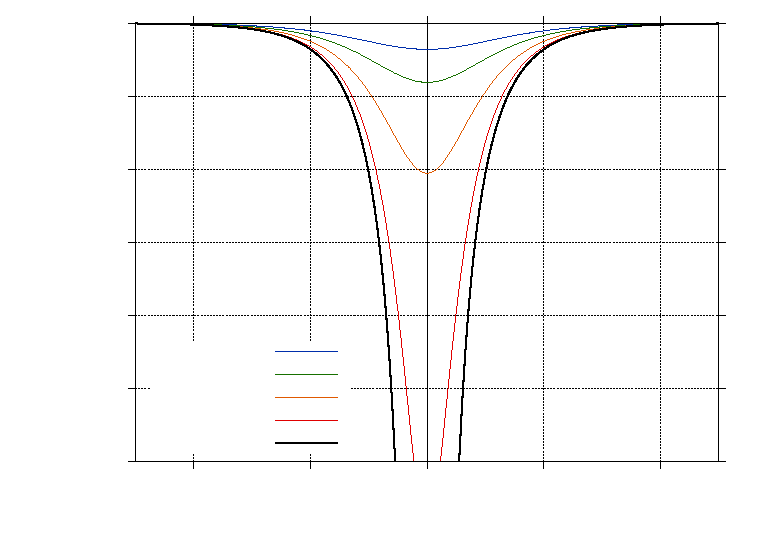
\includegraphics{Figures/twowires/InducedInteractionInterwireRealSpace/InducedInteraction}}%
    \gplfronttext
  \end{picture}%
\endgroup
  
\caption{The \textit{inter}wire induced interaction, $\tilde{V}^{12}_{\text{ind}}(x, 0)$, plotted as a function of $x$ for several values of the interwire distance, $d$. Coloured lines: for any nonzero interwire distance, the interaction is finite at the origin. Black line: the \textit{inter}- and \textit{intra}wire interactions coincide. \\ Parameters: $(n_Ba_B^3)^{1/3} = 0.01$, $(n_Ba_{BF}^3)^{1/3} = 0.1$, $l_t = 0$, $\frac{m_B}{m_F} = 7/40$, $\frac{n_F}{n_B^{1/3}} = 0.215$, $v_F/c_0 = 0.33$.}  
\label{fig.V12indx}  
\end{center}    
\end{figure}

In appendix \ref{Appendix.inducedinteraction.realspace} we calculate the real space induced interaction for general Matsubara frequencies $\omega_m = 2\pi m k_BT$ in the $l_t = 0$ limit. This general interaction is qualitatively the same as the zero frequency component.  

\subsection{Momentum space}
\label{subsec.inducedinteraction.momentumspace}
Later, we want to express the Hamiltonian in momentum space. In this section we therefore calculate the momentum space induced interaction. 

We start with the \textit{inter}wire interaction. In chapter \ref{Chapter4} we will see, that the relevant expression is simply the Fourier transform of the real space interaction. Therefore, we could go back to equation \eqref{eq.V12indXBEC} for $\omega_q = 0$. However, it is simpler to use the real space expression found in subsection \ref{subsec.inducedinteraction.realspace} and perform the Fourier transform explicitly. We get:
\begin{equation}
V_{\text{ind}}^{12}(q,0) = \int dx \; \text{e}^{-iqx}\tilde{V}_{\text{ind}}^{12}(x,0) = 2\int_0^\infty \cos(qx)\tilde{V}_{\text{ind}}^{12}(x,0), \nonumber
\end{equation}
since the induced interaction is even in real space. Writing the variables in units of the range $\xi/\sqrt{2}$:
\begin{equation}
V_{\text{ind}}^{12}(\tilde{q},0) = -\frac{2n_Bg^2_{BF}m_B}{\pi}\int_0^\infty d\tilde{x} \cos(\tilde{q}\tilde{x})\frac{ \text{e}^{ -\sqrt{\tilde{x}^2+\tilde{d}^2} } }{\sqrt{\tilde{x}^2+\tilde{d}^2}} = -\frac{2n_Bg^2_{BF}m_B}{\pi}K_0\left[\tilde{d}\sqrt{\tilde{q}^2+1}\right], \nonumber
\end{equation}
where $K_0(x)$ is the modified Bessel function of the second kind of order zero. This calculation is done with the use of the Fourier cosine transform routine in Maple 16. Since $\tilde{q} = \frac{q\xi}{\sqrt{2}}, \tilde{d} = \frac{\sqrt{2}d}{\xi}$, we finally get:
 \begin{equation}
V_{\text{ind}}^{12}(q,0) = -\frac{2n_Bg^2_{BF}m_B}{\pi}K_0\left[\sqrt{(qd)^2+\frac{2d^2}{\xi^2}}\right]. 
\label{eq.V12indq.zerofrequency}
\end{equation}
We hereby have a closed form expression for the interwire induced interaction in momentum space. 

Next we turn to the \textit{intra}wire interaction. The situation here is more tricky. As already noted, the induced interaction in equation \eqref{eq.V11indXBEC} diverges for $l_t \to 0$. However, in chapter \ref{Chapter4} we will see, that the antisymmetry of the fermionic operators leads to two terms for the interaction. One is the \textit{direct} term, $V^{11}_{\text{ind}}\left( p, 0 \right)$, the other is the \textit{exchange} term, $V^{11}_{\text{ind}}\left( k - q + p, 0 \right)$. Here $p$ is the momentum transfer and $k, q$ are the momenta of the incoming fermions. The resulting relevant interaction vertex is: 
\begin{equation}
W^{11}_{\text{ind}}(k, q, p) = \frac{1}{2} ( \underset{\text{Direct}}{\underbrace{V^{11}_{\text{ind}}\left( p, 0 \right)}} - \underset{\text{Exchange}}{\underbrace{V^{11}_\text{ind}\left( k - q + p, 0 \right) }} ). 
\label{eq.Wkqp.scattering.amplitude}
\end{equation}
We wish to calculate the very narrow wire width limit, $l_t \to 0$, of this expression. Going back to equation \eqref{eq.V11indXBEC} for $\omega_q = 0$, it turns out, that we can express $V^{11}_\text{ind}\left( q, 0 \right)$ as:
\begin{equation}
V^{11}_{\text{ind}}(q, 0) = -\frac{m_Bg_{BF}^2n_B}{\pi} \text{e}^{F(q)} E_1(F(q)),
\label{eq.V11indq.zerofrequency.ltnonzero}
\end{equation}
where $F(q) = \frac{l_t^2}{2}\left(q^2 + \frac{2}{\xi^2} \right)$ and $E_1(x)$ is the exponential integral: $E_1(x) = \int_1^\infty du \frac{\text{e}^{-xu}}{u}$. Inserting this into the above expression for $W^{11}_{\text{ind}}$ yields:
\begin{align}
W^{11}_{\text{ind}}(k, q, p) &= \frac{1}{2}\left[V^{11}_\text{ind}(p, 0) - V^{11}_\text{ind}(k - q + p, 0)\right] \nonumber \\
&= -\frac{m_Bg_{BF}^2n_B}{2\pi}\left[ \text{e}^{F(p)} E_1(F(p)) - \text{e}^{F(k - q + p)} E_1(F(k - q + p)) \right], \nonumber
\end{align}
Now we take the $l_t \to 0$ limit. We have $\partial_x E_1(x) = -\int_1^{\infty}du\; \text{e}^{-xu} = -\frac{1}{x}\text{e}^{-x}$. For $0 < x \ll 1$, this gives $\partial_xE_1(x) = -\frac{1}{x}$. Hence, in this regime we have $E_1(x) = C -\ln(x)$, where $C$ is a constant.\footnote{The constant is minus the Euler-Mascheroni constant $\gamma$. To ten digits precision $\gamma = 0.5772156649$. This is found in Maple 16.} The exponentials $\text{e}^{F(p)}$ and $\text{e}^{F(k - q + p)}$ just give $1$ in the $l_t \to 0$ limit, and so we are left with the expression:
\begin{equation}
\lim_{l_t \to 0} \; W^{11}_{\text{ind}}(k, q, p) = -\frac{m_Bg_{BF}^2n_B}{2\pi} \ln\left[\frac{(k - q + p)^2 + 2/\xi^2}{p^2 + 2/\xi^2}\right].
\label{eq.Wkqp.scattering.amplitude.lt=0} 
\end{equation}
Hereby we also have a closed form expression for the intrawire interaction in momentum space. The fact that we have these closed form expressions is crucial for the feasibility of the later numerical analyses.




